\documentclass[journal, a4paper]{IEEEtran}

% some very useful LaTeX packages include:
\usepackage[brazil]{babel}
\usepackage[utf8x]{inputenc}
\usepackage{amsmath}
\usepackage{float}
\usepackage{mathtools}
\usepackage{natbib}

%\usepackage{cite}      % Written by Donald Arseneau
                        % V1.6 and later of IEEEtran pre-defines the format
                        % of the cite.sty package \cite{} output to follow
                        % that of IEEE. Loading the cite package will
                        % result in citation numbers being automatically
                        % sorted and properly "ranged". i.e.,
                        % [1], [9], [2], [7], [5], [6]
                        % (without using cite.sty)
                        % will become:
                        % [1], [2], [5]--[7], [9] (using cite.sty)
                        % cite.sty's \cite will automatically add leading
                        % space, if needed. Use cite.sty's noadjust option
                        % (cite.sty V3.8 and later) if you want to turn this
                        % off. cite.sty is already installed on most LaTeX
                        % systems. The latest version can be obtained at:
                        % http://www.ctan.org/tex-archive/macros/latex/contrib/supported/cite/

\usepackage{graphicx}   % Written by David Carlisle and Sebastian Rahtz
                        % Required if you want graphics, photos, etc.
                        % graphicx.sty is already installed on most LaTeX
                        % systems. The latest version and documentation can
                        % be obtained at:
                        % http://www.ctan.org/tex-archive/macros/latex/required/graphics/
                        % Another good source of documentation is "Using
                        % Imported Graphics in LaTeX2e" by Keith Reckdahl
                        % which can be found as esplatex.ps and epslatex.pdf
                        % at: http://www.ctan.org/tex-archive/info/

\usepackage{psfrag}    % Written by Craig Barratt, Michael C. Grant,
                        % and David Carlisle
                        % This package allows you to substitute LaTeX
                        % commands for text in imported EPS graphic files.
                        % In this way, LaTeX symbols can be placed into
                        % graphics that have been generated by other
                        % applications. You must use latex->dvips->ps2pdf
                        % workflow (not direct pdf output from pdflatex) if
                        % you wish to use this capability because it works
                        % via some PostScript tricks. Alternatively, the
                        % graphics could be processed as separate files via
                        % psfrag and dvips, then converted to PDF for
                        % inclusion in the main file which uses pdflatex.
                        % Docs are in "The PSfrag System" by Michael C. Grant
                        % and David Carlisle. There is also some information
                        % about using psfrag in "Using Imported Graphics in
                        % LaTeX2e" by Keith Reckdahl which documents the
                        % graphicx package (see above). The psfrag package
                        % and documentation can be obtained at:
                        % http://www.ctan.org/tex-archive/macros/latex/contrib/supported/psfrag/

%\usepackage{subfigure} % Written by Steven Douglas Cochran
                        % This package makes it easy to put subfigures
                        % in your figures. i.e., "figure 1a and 1b"
                        % Docs are in "Using Imported Graphics in LaTeX2e"
                        % by Keith Reckdahl which also documents the graphicx
                        % package (see above). subfigure.sty is already
                        % installed on most LaTeX systems. The latest version
                        % and documentation can be obtained at:
                        % http://www.ctan.org/tex-archive/macros/latex/contrib/supported/subfigure/

\usepackage{url}        % Written by Donald Arseneau
                        % Provides better support for handling and breaking
                        % URLs. url.sty is already installed on most LaTeX
                        % systems. The latest version can be obtained at:
                        % http://www.ctan.org/tex-archive/macros/latex/contrib/other/misc/
                        % Read the url.sty source comments for usage information.

%\usepackage{stfloats}  % Written by Sigitas Tolusis
                        % Gives LaTeX2e the ability to do double column
                        % floats at the bottom of the page as well as the top.
                        % (e.g., "\begin{figure*}[!b]" is not normally
                        % possible in LaTeX2e). This is an invasive package
                        % which rewrites many portions of the LaTeX2e output
                        % routines. It may not work with other packages that
                        % modify the LaTeX2e output routine and/or with other
                        % versions of LaTeX. The latest version and
                        % documentation can be obtained at:
                        % http://www.ctan.org/tex-archive/macros/latex/contrib/supported/sttools/
                        % Documentation is contained in the stfloats.sty
                        % comments as well as in the presfull.pdf file.
                        % Do not use the stfloats baselinefloat ability as
                        % IEEE does not allow \baselineskip to stretch.
                        % Authors submitting work to the IEEE should note
                        % that IEEE rarely uses double column equations and
                        % that authors should try to avoid such use.
                        % Do not be tempted to use the cuted.sty or
                        % midfloat.sty package (by the same author) as IEEE
                        % does not format its papers in such ways.

\usepackage{amsmath}    % From the American Mathematical Society
                        % A popular package that provides many helpful commands
                        % for dealing with mathematics. Note that the AMSmath
                        % package sets \interdisplaylinepenalty to 10000 thus
                        % preventing page breaks from occurring within multiline
                        % equations. Use:
%\interdisplaylinepenalty=2500
                        % after loading amsmath to restore such page breaks
                        % as IEEEtran.cls normally does. amsmath.sty is already
                        % installed on most LaTeX systems. The latest version
                        % and documentation can be obtained at:
                        % http://www.ctan.org/tex-archive/macros/latex/required/amslatex/math/



% Other popular packages for formatting tables and equations include:

%\usepackage{array}
% Frank Mittelbach's and David Carlisle's array.sty which improves the
% LaTeX2e array and tabular environments to provide better appearances and
% additional user controls. array.sty is already installed on most systems.
% The latest version and documentation can be obtained at:
% http://www.ctan.org/tex-archive/macros/latex/required/tools/

% V1.6 of IEEEtran contains the IEEEeqnarray family of commands that can
% be used to generate multiline equations as well as matrices, tables, etc.

% Also of notable interest:
% Scott Pakin's eqparbox package for creating (automatically sized) equal
% width boxes. Available:
% http://www.ctan.org/tex-archive/macros/latex/contrib/supported/eqparbox/

% *** Do not adjust lengths that control margins, column widths, etc. ***
% *** Do not use packages that alter fonts (such as pslatex).         ***
% There should be no need to do such things with IEEEtran.cls V1.6 and later.


% Your document starts here!
\begin{document}

% Define document title and author
	\title{Relatório de Classificação de Padrões}
	\author{Victor Carreira
	\thanks{Professora: Marley. Eng. Elétrica. PUC-RIO}}
	\markboth{Trabalho 01}{}
	\maketitle

% Write abstract here
\begin{abstract}
	Este relatório apresenta o resultado de sete testes conduzidos em uma rede neural artificial \textit{Perceptron multi-camadas} em um banco de dados de uma instituição financeira com o intuito de se fazer uma análise de crédito bancário.  A base de dados contém 2077 exemplos de créditos concedidos. Possui 11 atributos de entrada e 2 classes de saída. A saída da rede indica se o cliente pagou o empréstimo ou não. Os resultados dos testes estão apresentados em formato de tabela.
\end{abstract}

% Each section begins with a \section{title} command
\section{Introdução}
    As Redes Neurais Artificiais (RNA) são inspiradas em modelos sensoriais do processamento de tarefas realizadas pelo cérebro \citep{Hagan1996}. Uma RNA, portanto pode ser criada através da aplicação de algoritmos matemáticos que imitem a tarefa realizada por um neurônio \citep{Nedjah2016}. Uma rede neural artificial possui semelhanças com a rede biológica presente no sistema nervoso central, neste o cômputo de informações realizado do cérebro é feito através de uma vasta quantidade de neurônios interconectados \citep{Feldman1988,Poulton2002}. A comunicação entre essas células é realizada através de impulsos elétricos. Estes são transmitidos e recebidos por meio de sinapses nervosas entre axônios e dendritos. As sinapses são estruturas elementares e uma unidade funcional localizada entre dois neurônios \citep{Krogh2008}.

	\citet{McCulloch1943} redigem o trabalho pioneiro onde foi modelado um neurônio cuja resposta dependia do \textit{input}\footnote{Valor de entrada} que provinha de outros neurônios e do peso utilizado.  Já \citet{Rosenblatt1962} cria a teoria de convergência do \textit{Perceptron} onde ele prova que modelos de neurônios possuem propriedades similares ao cérebro humano \citep{Kanal2001}. Neste sentido as rede neuronais artificiais podem realizar performasses sofisticadas no reconhecimento de padrões, mesmo se alguns neurônios forem destruídos \citep{Levy1997}. \citet{Minsky1969} demonstraram que \textit{Perceptrons} somente resolvem uma classe muito limitada de problemas que podem ser linearizados.

% Main Part
\section{Objetivo e Metodologia}


Uma instituição financeira possui uma base de dados com o histórico de crediário
oferecido aos seus clientes. Baseado neste histórico, a instituição deseja inferir se um
novo cliente pagará ou não a dívida contraída.

A base de dados possui $2077$ exemplos, com $11$ atributos cada, de créditos concedidos
aos seus clientes. A base informa ainda se o cliente honrou ou não o pagamento do
empréstimo. 

A partir da base original, foram criadas 3 bases de treinamento, com $1500$ exemplos
cada escolhidos aleatoriamente a partir da base original, e $3$ bases de testes com $577$
exemplos cada, representando, respectivamente, $72,2\%$ e $27,8\%$ do total de cada sub-
grupos de dados. Estas bases estão nos arquivos treino01.txt, treino02.txt, treino03.txt,
teste01.txt, teste02.txt e teste03.txt. Utilizar o software WEKA, para criar um classificador, baseado em redes neurais, capaz de informar se um novo cliente será potencialmente adimplente ou não. 

Abra cada um dos arquivos no WEKA e grave-os em formato .arff. Através de um
editor de textos (por exemplo, o WordPad), altere o tipo associado às variáveis
categóricas conforme o exemplo \textit{@attribute NDEP numeric ⇒ @attribute NDEP {0,1,2,3,4,5,6,7}}

 Para cada uma das configurações abaixo, apresente os resultados para cada par de conjuntos de treino e de teste, assim como a média e o desvio padrão dos 3 pares: I, II, III, IV, V, VI.
\begin{itemize}
	 \item Sem normalização dos atributos de entrada;
     \item Com normalização dos atributos de entrada e SEM codificação binária dos atributos categóricos;
     \item Com normalização e codificação binária dos atributos categóricos de entrada e com 2 números diferentes de neurônios na camada escondida;
     \item Com normalização dos atributos de entrada e variando o número de épocas durante a fase de treinamento. Escolha 3 durações de treino diferentes (por exemplo: 1, 100 e 1000);
     \item Com normalização dos atributos de entrada e utilizando um conjunto de validação;
     \item Tente obter melhores resultados (se possível) agrupando algumas categorias das variáveis ESTC e NDEP. Para isto, utilize o filtro não supervisionado MergeTwoValues.
\end{itemize}

Para os itens I, II, IV, V e VI, indique para cada um dos casos o número de neurônio na
camada escondida e explique a sua escolha. Para todos os itens, não varie a taxa de
aprendizagem nem o termo de momento.



\section{Princípio Teórico}
O neurônio de \citet{McCulloch1943} propõe um limite binário para a criação de um modelo. Este neurônio artificial registra uma soma de pesos de $n$ sinais de entrada, $x_{j}$, $j=1,2,3,...,n$, e fornece um \textit{output}\footnote{Valor de saída} de $1$ caso esta soma esteja acima do limite $u$. Caso contrário o \textit{output} é $0$. Matematicamente essa relação pode ser descrita de acordo com a Eq. \ref{Eq.neuronio-McCulloch}:

\begin{eqnarray}
y=\theta \left( \sum^{n}_{j=1} w_{j} x_{j} -u \right)
\label{Eq.neuronio-McCulloch}
\end{eqnarray}

Onde $\theta$ é o passo dado na posição $0$, $w_{j}$ é chamada sinapse-peso associado a um $j_{esimo}$ \textit{input}. A título de simplificação a função limite\footnote{Genericamente chamada de função de ativação} $u$ é considerada um outro peso $w_{0}=-u$ anexado a um neurônio com um \textit{input} constante $x_{0}=1$. Pesos positivos correspondem a uma sinapse \textbf{excitatória}, enquanto pesos negativos correspondem a uma sinapse \textbf{inibitória}. Este modelo contém uma série de simplificações que não refletem o verdadeiro comportamento dos neurônios biológicos \citep{Mao1996}.  

Derivações do neurônio de \citet{McCulloch1943} na escolha das funções de ativação. Uma função largamente utilizada é a função sigmóide, que exibe uma suavização dos \textit{outputs} a medida que o valor da função diminui \citep{Mao1996,Misra2010}. Essa função de ativação pode ser expressa de acordo com a Eq. \ref{f.sigmoide}:

\begin{eqnarray}
g(x)=1/(1+e^{-\beta x})
\label{f.sigmoide}
\end{eqnarray}

Onde $\beta$ é o parâmetro de inclinação. A Fig. \ref{Esquematico de McCulloch} ilustra a sequência lógica da operação de uma RNA para um neurônio simples de McCulloch-Pitts. 
\\
\begin{figure}[H]
	\centering
	\setlength{\fboxsep}{8pt}
	\setlength{\fboxrule}{0.1pt}
	\fbox{
		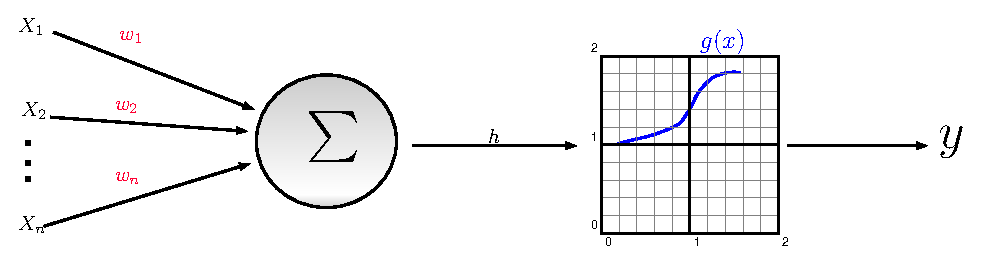
\includegraphics[scale=0.4]{Images/McCulloch.eps}
	}
	\caption{Modelo esquemático de um neurônio de McCulloch-Pitts. Onde $x_{1}, x_{2}, ..., x_{n}$ são os \textit{inputs}, $w_{1}, w_{2}, ..., w_{n}$ são os pesos, h é o treino, $g(x)$ é a função de ativação, e $y$ é o \textit{output}.}
	\label{Esquematico de McCulloch}
\end{figure}

As redes alimentadas diretamente são aquelas redes cujos grafos orientados se distinguem pela presença de um ou mais camadas ocultas e cujos nós são chamados de neurônios ocultos. A função do neurônio é intervir entre a camada externa e a saída da rede de maneira útil. Adicionando-se camadas ocultas a rede torna-se capaz de realizar estatísticas de ordem elevada \citep{Haykin1999}.


\section{Resultados}

A tabela \ref{grupo01} refere-se ao conjunto de $6$ testes realizados no primeiro banco de dados que é uma composição dos dados de treinamento e testes $1$. Os testes utilizados neste trabalho foram em sua totalidade compostos por $2$ camadas ocultas. O número de neurônios ocultos estão indicados nas tabelas, como Neurônios na CO1 (camada oculta 1) e como Neurônios na CO2 (camada oculta 2).

\begin{table}[H]
	\begin{center}
				\caption{Grupo $01$}
				\label{grupo01}
				\begin{tabular}{|c|c|c|c|c|c|c|}\hline	
					\textbf{Configuração} &\textbf{I}&\textbf{II}&\textbf{III}&\textbf{IV}&\textbf{V}&\textbf{VI} \\ \hline 
					{Neuronios na CO1} & 4 & 4 & 4 & - & 4 & 4 \\ \hline
					{Neuronios na CO2} & 4 & 4 & 2 & - & 4 & 4 \\ \hline
					{Cl. Correta (\%)} & 52.3 & 91.3 & 91.2  & - & 52.3 &  97 \\ \hline
					{Cl. Incorreta (\%)} & 47.7 & 8.7 & 8.8 & - & 47.7 & 3 \\ \hline
					{MAE (\%)} & 0.49 &  0.13 & 0.14 & - & 0.49 & 0.04 \\ \hline
					{RMSE (\%)} & 0.50 & 0.26 & 0.27 & - & 0.49 & 0.17 \\ \hline
					{RAE (\%)} & 99.68 & 26.23 & 28.3 & - & 100.2 & 8.50 \\ \hline
					{RRSE(\%)} & 100.23 & 52.23 & 53.75 & - & 100.1 & 36.51 \\ \hline
					{Dados Totais} & 1500 & 1500  & 1500 & - & 1500 & 100 \\ \hline
				\end{tabular}  
	\end{center}
\end{table}

A tabela \ref{grupo01IV} refere-se os testes de variações de épocas do conjunto de dados $1$.

\begin{table}[H]
	\begin{center}
		\caption{Grupo $01$: variando as épocas no teste IV}
		\label{grupo01IV}
		\begin{tabular}{|c|c|c|c|}\hline	
			\textbf{Configuração} &$\textbf{IV}_{1}$&$\textbf{IV}_{100}$&$\textbf{IV}_{1000}$ \\ \hline 
			{Neuronios na CO1}   & 4      & 4     & 4      \\ \hline
			{Neuronios na CO2}   & 4      & 4     & 4      \\ \hline
			{Cl. Correta (\%)}   & 52.3   & 90.8  & 91.53  \\ \hline
			{Cl. Incorreta (\%)} & 47.7   & 9.2   & 8.47   \\ \hline
			{MAE (\%)}           & 0.49   & 0.16  & 0.14   \\ \hline
			{RMSE (\%)}          & 0.51   & 0.27  & 0.26   \\ \hline
			{RAE (\%)}           & 99.63  & 32.34 & 27.49   \\ \hline
			{RRSE(\%)}           & 100.23 & 54.49 & 52.89  \\ \hline
			{Dados Totais}       & 1500   & 1500  & 1500   \\ \hline
		\end{tabular}  
	\end{center}
\end{table}

Aqui iniciam-se o conjunto de testes 2. 

\begin{table}[H]
	\begin{center}
		\caption{Grupo $02$}
		\label{grupo02}
		\begin{tabular}{|c|c|c|c|c|c|c|}\hline	
			\textbf{Configuração} &\textbf{I}&\textbf{II}&\textbf{III}&\textbf{IV}&\textbf{V}&\textbf{VI} \\ \hline 
			{Neuronios na CO1} & 4 & 4 & 4 & - & 4 & 4 \\ \hline
			{Neuronios na CO2} & 4 & 4 & 8 & - & 4 & 4 \\ \hline
			{Cl. Correta (\%)} & 53.2667 & 91.4667 & 91.6667  & - & 53.2667 &  91.8667 \\ \hline
			{Cl. Incorreta (\%)} & 46.7333 & 8.5333 & 8.3333 & - & 46.7333 & 8.1333 \\ \hline
			{MAE (\%)} & 0.4927 &  0.1247 & 0.1213 & - & 0.4999 & 0.1165 \\ \hline
			{RMSE (\%)} &0.5052 & 0.2637 & 0.2657 & - & 0.4999 & 0.2584 \\ \hline
			{RAE (\%)} & 98.9582 & 25.0564 & 24.3633 & - & 100.4037 & 23.3909 \\ \hline
			{RRSE(\%)} & 101.2566 & 52.8491 & 53.2471 & - & 100.1905 & 51.7846 \\ \hline
			{Dados Totais} & 1500 & 1500  & 1500 & - & 1500 & 1500 \\ \hline
		\end{tabular}  
	\end{center}
\end{table}

Variações das épocas do conjunto de testes 2. 

\begin{table}[H]
	\begin{center}
		\caption{Grupo $02$: variando as épocas no teste IV}
		\label{grupo02IV}
		\begin{tabular}{|c|c|c|c|}\hline	
			\textbf{Configuração} &$\textbf{IV}_{1}$&$\textbf{IV}_{100}$&$\textbf{IV}_{1000}$ \\ \hline 
			{Neuronios na CO1}   & 4      & 4     & 4      \\ \hline
			{Neuronios na CO2}   & 4      & 4     & 4      \\ \hline
			{Cl. Correta (\%)}   & 53.2667   & 91.4   & 91.8667  \\ \hline
			{Cl. Incorreta (\%)} & 46.7333   & 8.6    & 8.1333   \\ \hline
			{MAE (\%)}           & 0.4913   & 0.1384  & 0.1165   \\ \hline
			{RMSE (\%)}          & 0.5083   & 0.2669  & 0.2584   \\ \hline
			{RAE (\%)}           & 98.6867 & 27.807 & 23.3909   \\ \hline
			{RRSE(\%)}           & 101.8876 & 53.4966 & 51.7846  \\ \hline
			{Dados Totais}       & 1500   & 1500  & 1500   \\ \hline
		\end{tabular}  
	\end{center}
\end{table}

Aqui iniciam-se o conjunto de testes 3. 

\begin{table}[H]
	\begin{center}
		\caption{Grupo $03$}
		\label{grupo03}
		\begin{tabular}{|c|c|c|c|c|c|c|}\hline	
			\textbf{Configuração} &\textbf{I}&\textbf{II}&\textbf{III}&\textbf{IV}&\textbf{V}&\textbf{VI} \\ \hline 
			{Neuronios na CO1} & 4 & 4 & 1 & - & 4 & 4 \\ \hline
			{Neuronios na CO2} & 4 & 4 & 12 & - & 4 & 4 \\ \hline
			{Cl. Correta (\%)} & 49  & 91.4  & 90.8667  & - & 51 &  66 \\ \hline
			{Cl. Incorreta (\%)} & 51  & 8.6 & 9.1333 & - & 49 & 34 \\ \hline
			{MAE (\%)} & 0.5006 &  0.1228 & 0.1638 & - & 0.5  &  0.4979 \\ \hline
			{RMSE (\%)} & 0.5013 & 0.2654 & 0.2783 & - & 0.5 & 0.4979 \\ \hline
			{RAE (\%)} & 100.151 & 24.5646 & 32.7792 & - & 100.0321 & 110.5297 \\ \hline
			{RRSE(\%)} & 100.2846 & 53.0866 & 55.6619 & - & 100.0128 & 104.9763 \\ \hline
			{Dados Totais} & 1500 & 1500  & 1500 & - & 1500 & 100 \\ \hline
		\end{tabular}  
	\end{center}
\end{table}

Aqui seguem os testes de variação de épocas. 

\begin{table}[H]
	\begin{center}
		\caption{Grupo $03$: variando as épocas no teste IV}
		\label{grupo03IV}
		\begin{tabular}{|c|c|c|c|}\hline	
			\textbf{Configuração} &$\textbf{IV}_{1}$&$\textbf{IV}_{100}$&$\textbf{IV}_{1000}$ \\ \hline 
			{Neuronios na CO1}   & 4      & 4     & 4      \\ \hline
			{Neuronios na CO2}   & 4      & 4     & 4      \\ \hline
			{Cl. Correta (\%)}   & 49    & 90.3333  & 91  \\ \hline
			{Cl. Incorreta (\%)} & 51    & 9.6667   & 9   \\ \hline
			{MAE (\%)}           & 0.5002   & 0.1321  & 0.1318   \\ \hline
			{RMSE (\%)}          & 0.5004   & 0.2748  & 0.2653   \\ \hline
			{RAE (\%)}           & 100.0891  & 26.4304 & 26.3714   \\ \hline
			{RRSE(\%)}           & 100.099 & 54.9758 & 53.0768  \\ \hline
			{Dados Totais}       & 1500   & 1500  & 1500   \\ \hline
		\end{tabular}  
	\end{center}
\end{table}





\section{Conclusões}
	Ao analisar previamente os dados é possível que o número de dependentes NDEP é majoritariamente composto por uma pessoa

% Now we need a bibliography:


\bibliographystyle{apalike}
\bibliography{references}


% Your document ends here!
\end{document}